\documentclass[sigconf,nonacm]{acmart}
\usepackage[utf8]{inputenc}
\usepackage{pgfplots}
\usepackage{subcaption}
\usepackage{adjustbox}
\usepackage{mathtools}
\usepackage{graphicx}
\usepackage{url}
\usepackage{minted}


\usetikzlibrary{
    patterns,
    chains,
    backgrounds,
    calc,
    shadings,
    shapes.arrows,
    arrows,
    shapes.symbols,
    shadows,
    positioning,
    decorations.markings,
    backgrounds,
    arrows.meta,
    external
}
\usepackage{array}

\DeclareUnicodeCharacter{2212}{−}
\usepgfplotslibrary{groupplots,dateplot}
\usetikzlibrary{patterns,shapes.arrows}
\pgfplotsset{compat=newest}

\newcommand{\code}[1]{\texttt{#1}}

\newif\iffinal

\iffinal
  \newcommand{\max}[1]{}
  \newcommand{\ryan}[1]{}
  \newcommand{\todo}[1]{}
\else
  \newcommand{\max}[1]{{\textcolor{red}{ Max: #1 }}}
  \newcommand{\ryan}[1]{{\textcolor{magenta}{ Ryan: #1 }}}
  \newcommand{\todo}[1]{{\textcolor{blue}{ TODO: #1 }}}
  

\fi


\begin{document}

\title{Ultrafast focus detection using multi-scale histologic features}


\author{Maksim Levental}
\affiliation{\institution{University of Chicago}}
\author{Ryan Chard}
\affiliation{\institution{Argonne National Laboratory}}
\author{Gregg A. Wildenberg}
\affiliation{\institution{University of Chicago}}

\begin{abstract}
    We present a fast out-of-focus detection algorithm for electron microscopy images collected serially. 
    Such images are collected for the purposes of post-processing tasks such as montaging, alignment, and image segmentation. 
    Such an algorithm is necessitated by recent increases in collection rates owing to advances in microscopy technology. 
    Our technique adapts classical computer vision and is based on detecting various fine-grained histologic features. 
    We further exploit the inherent parallelism in the technique by employing GPGPU primitives in order to accelerate characterization. 
    Tests are performed that demonstrate faster than real time detection of out-of-focus conditions. 
    <We also deploy to funcX something something>.
    We discuss extensions that enable scaling out to support multi-beam microscopes and integration with existing focus systems for purposes of implementing auto-focus.

\end{abstract}

\maketitle

\section{Introduction}\label{sec:intro}

Advancements in the automation of serial scanning electron microscopy (SEM)  impose a regime where thousands, if not tens of thousands, of images can now be automatically collected by researchers.
\todo{<bio use cases>}
This puts greater demand on conventional auto-focus algorithms for ensuring each image is in focus, as an alternative to the user manually evaluating each image by eye. 
Without such algorithms, critical bottlenecks are created where the user is forced to reacquire individual, deficient (out-of-focus), images and manually reinsert them into the sequence of thousands of other images already acquired.
This is an onerous task which requires taking into account alignment and boundary overlap. 
Furthermore, failure to quickly identify and reacquire deficient images negatively impacts the accuracy of downstream, post-processing; for example 2D montaging, 3D alignment, or automatic segmentation pipelines. 
While many microscopes have builtin auto-focus algorithms, these often fail to achieve acceptable accuracy due to intrinsic mediating factors (e.g. stage drift) and extrinsic mediating factors (e.g. sample artifacts, non-uniformity in the sample). 

Auto-focus technology is a critical component of many imaging systems; from consumer cameras (for purposes of convenience) to industrial inspection tools to scientific instrumentation.
Such technology is typically either active or passive; active methods exploit some auxiliary device or mechanism to measure the distance of the optics from the scene, while passive methods analyze the definition of sharpness of an image by virtue of some proxy measure. 
Here we focus on passive methods, as we explicitly aim to augment existing microscopy equipment without the need for costly and complex retrofitting.

Passive proxies for the degree-of-focus (DOF) include the energy of the Laplacian, discrete cosine transform, or weighted histogram of an image; for effecting a high DOF a search can be performed.
When used as a component of an auto-focus system (as opposed to OOF detection system) all such passive methods are unsuitable for the purpose of real-time (or even near-real-time) characterization of DOF due to their long scanning times (multiple images need to be collected at potentially different depths).
As our method currently aims only to detect OOF events we do not consider or implement any focus search techniques (but do describe plans for such future work).

To overcome these challenges, thereby ensuring that images are faithfully acquired, we propose a method to evaluate image definition based multi-scale histologic feature detection (MHD). 
By multi-scale histologic feature detection we mean the resolving and characterization of histological structure at multiple length scales; for our particular use-case this means structures ranging from cell walls to whole organelles.
The key insight being that the ability to resolve structure across the range of feature scales is highly correlated with a high-definition, i.e. in-focus, image.

Due to limitations of the extensibility of commercial microscopy equipment, we do not aim here to directly implement auto-focusing.
Rather than focusing the microscope, as auto-focusing algorithms would, our algorithm operates downstream of collection and reports out-of-focus (OOF) events to the user. 
This enables the user to intervene and initiate reacquisition protocols (on the microscope) before unknowingly proceeding with collecting the next series of images or proceeding with downstream image processing and analysis. 
This human-in-the-loop remediation protocol already saves the user much wasted collection time and tedium in triaging defective collection runs.

This rest of this article is organized as follows: section \ref{sec:mhd} describes our focus detection method in the abstract, section \ref{sec:implementation} discusses optimizations made in order to achieve real-time performance with our method, section \ref{sec:evaluation} reports results of evaluating our method on sequences of images collected at varying focus depths, section \ref{sec:related} discusses related work and how our work is distinct therefrom, and finally section \ref{sec:conclusion} concludes with a discussion of future research.

\section{Gregg sells science!}

TYPE HERE

\section{Multi-scale Histologic Feature Detection}\label{sec:mhd}

We base our multi-scale histologic feature detection on classic on scale-space representations of signals. 
We give a brief overview (a more comprehensive discussion is available~\cite{}) and describe our adaptation.

The fundamental principle of scale-space feature detection is that natural images possess structure at multiple scales and that features at a particular scale can be characterized in isolation of features at other scales.
Typically characterization is effected by convolution with a filter that satisfies the constraints of non-enhancement of local extrema, scale invariance and rotational invariance (along with some others~\cite{}).
One such filter~\cite{} is the symmetric, mean zero, 2D, Gaussian filter 
$$
G(x,y,\sigma) \coloneqq \frac{1}{2\pi \sigma^2} e^{-\frac{x^2 +y ^2}{2\sigma^2}}
$$
Thus, define the scale-space representation $L(x,y, t)$ of an image $I(x,y)$ to be the convolution of that image with a mean zero Gaussian filter:
$$
L(x,y,t) \coloneqq G(x,y,t) * I(x,y)
$$
where $t$ is the standard deviation of the Gaussian and determines the \textit{scale} of $L(x,y,t)$.
$L(x,y,t)$ has the interpretation that image one-dimensional structures of scale smaller than $\sqrt{t^2} = t$ have been removed due to blurring.
This is due to the fact that the variance of the Gaussian filter is $t^2$ and features of this scale are therefore "beneath the noise floor" of the filter or, in effect, suppressed by filtering procedure.
A corollary is that features with length scale $t$ will have maximal response being filtered by $G(x,y,t)$; for $t' < t$ smaller length scale features will dominate the response and for $t'' > t$, as already mentioned, the response will have been suppressed. 
Hence, at various scales $t$ we can use linear and non-linear combinations of space derivatives $\partial_x, \partial_y$ and derivatives in the scale $\partial_t$ to construct scale-invariant feature detectors; such feature detectors detect features such as corners, edges, and ridges.
For example, the zeros in scale of the scale normalized Laplacian 
\begin{equation}
    \partial_t \nabla^2 L \coloneqq \partial_t \left( \partial_x^2 + \partial _y^2\right) L = 0
    \label{eqn:blobdetector}
\end{equation}
correspond to uniform region (otherwise known as blobs) detectors.

\section{Implementation}\label{sec:implementation}

\begin{figure}
     \centering
     \begin{subfigure}[b]{0.5\textwidth}
         \centering
         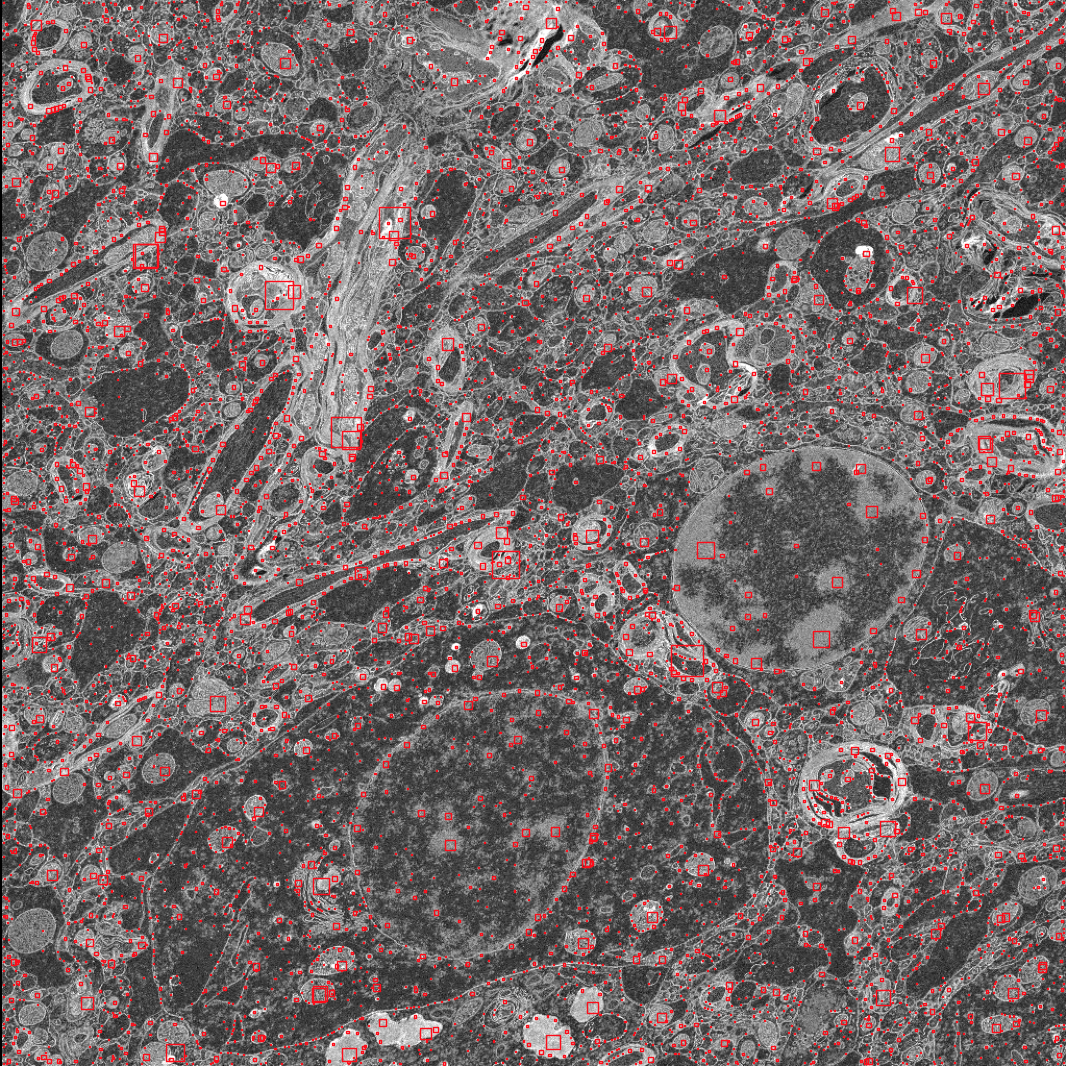
\includegraphics[width=1\linewidth]{in_focus.png}
         \caption{Histologic features of an in-focus section.}
         \label{subfig:infocus}
     \end{subfigure}
     \par\bigskip
     \begin{subfigure}[b]{0.5\textwidth}
         \centering
        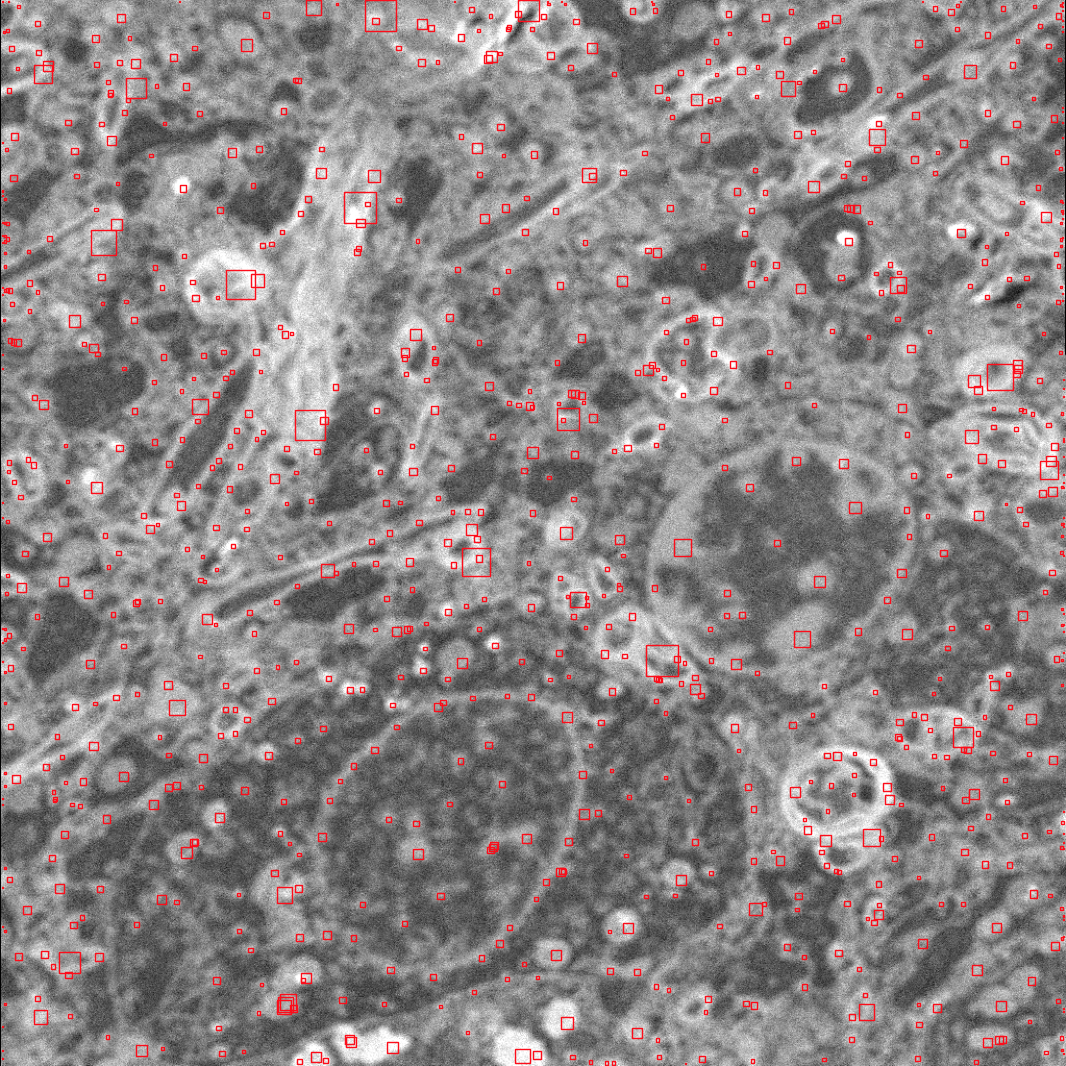
\includegraphics[width=1\linewidth]{out_of_focus.png}
         \caption{Histologic features of an out-of-focus section.}
         \label{subfig:outoffocus}
     \end{subfigure}
     \caption{Comparison of sections with histologic feature recognition as a function of focal depth.}
    \label{fig:histfeatsimages}
\end{figure}

We therefore propose to use a feature detector as a proxy for DOF, reasoning that quantity of features detected is positively correlated with DOF (see figure~\ref{fig:histfeatsimages}). 
To this end, we develop a feature detector based on eqn.~\ref{eqn:blobdetector} but optimized for latency (rather than for accuracy).
In order to verify our hypothesis we compare the number of histologic features detected as a function of absolute deviation from in-focus ($\lvert f - f' \rvert$ where $f'$ is the correct focal depth) for a series of sections with known focal depth (see figure~\ref{subfig:degreeoofcurve}). 
We observe a very strong log-linear relationship (see figure~\ref{subfig:degreeooffit}). 
Fitting such a log-linear relationship produces a line with $r=-0.9754$, confirming our hypothesis that quantity of histologic features detected is a good proxy measure for DOF.

\begin{figure}
     \centering
     \begin{subfigure}[b]{0.5\textwidth}
         \centering
         % This file was created by tikzplotlib v0.9.8.
\begin{tikzpicture}[trim axis left,trim axis right]

\definecolor{color0}{rgb}{0.12156862745098,0.466666666666667,0.705882352941177}

\begin{axis}[
scaled y ticks=base 10:-3,
legend cell align={left},
legend style={fill opacity=0.8, draw opacity=1, text opacity=1, draw=white!80!black},
tick align=outside,
tick pos=left,
% title={Feature count vs. OOF},
x grid style={white!69.0196078431373!black},
xlabel={Degree of OOF},
xmin=-1.09892007559144e-06, xmax=2.31000189170211e-05,
xtick style={color=black},
xmajorgrids,
ymajorgrids,
y grid style={white!69.0196078431373!black},
ylabel={\# features},
ymin=99.9931235536055, ymax=9059.85673521721,
ytick style={color=black},
% y tick label style={/pgf/number format/sci}
]
\addplot [draw=color0, fill=color0, forget plot, mark=*, mark size=1, only marks, mark options={solid,fill opacity=0}]
table{%
x  y
2.89713740402389e-08 7023
1.79997717738205e-05 977
9.99997577071001e-06 1882
2.00011560321043e-06 6755
6.00014606118044e-06 4607
1.20001917481398e-05 2045
2.19998022317905e-05 743
1.99991485475958e-06 6791
3.99993008374979e-06 5606
5.99994531274e-06 3664
1.80000366866596e-05 899
2.00000519156498e-05 798
8.00016129016978e-06 3590
1.000017651916e-05 2672
1.400020697713e-05 1644
1.99997870028003e-05 874
7.99996054173021e-06 2513
1.40000062286896e-05 1233
1.60002222061202e-05 1185
1.19999909997002e-05 1419
1.60000214576702e-05 1056
4.00013083219977e-06 5610
2.20000671446296e-05 728
1.400020697713e-05 1172
3.99993008374979e-06 6308
7.99996054173021e-06 2688
9.99997577071001e-06 2037
1.03169680003984e-09 7000
1.000017651916e-05 1794
2.19998022317905e-05 741
1.99991485475958e-06 6987
5.99994531274e-06 4299
1.40000062286896e-05 1291
1.80000366866596e-05 988
2.00011560321043e-06 6389
4.00013083219977e-06 4785
6.00014606118044e-06 3080
8.00016129016978e-06 2329
1.20001917481398e-05 1472
1.60002222061202e-05 995
1.79997717738205e-05 882
1.19999909997002e-05 1595
1.60000214576702e-05 1103
2.00000519156498e-05 847
2.20000671446296e-05 781
1.99997870028003e-05 798
1.14187389609749e-07 8645
1.74120792746993e-06 8487
4.00013083219977e-06 5997
2.19998022317905e-05 831
1.99991485475958e-06 8516
3.99993008374979e-06 6280
9.99997577071001e-06 2037
1.80000366866596e-05 1004
6.00014606118044e-06 3510
8.00016129016978e-06 2658
1.20001917481398e-05 1517
1.60002222061202e-05 1095
7.99996054173021e-06 2740
2.00000519156498e-05 888
1.000017651916e-05 1958
1.79997717738205e-05 1022
1.99997870028003e-05 899
1.19999909997002e-05 1634
1.40000062286896e-05 1333
1.60000214576702e-05 1118
1.400020697713e-05 1253
5.99994531274e-06 3899
};
% \addplot [semithick, red]
% table {%
% 1.03169680003984e-09 8652.59020741432
% 2.89713740402389e-08 8621.47458132233
% 1.14187389609749e-07 8527.26131703851
% 1.74120792746993e-06 6913.51092038955
% 1.99991485475958e-06 6686.69355019204
% 1.99991485475958e-06 6686.69355019204
% 1.99991485475958e-06 6686.69355019204
% 2.00011560321043e-06 6686.52046851991
% 2.00011560321043e-06 6686.52046851991
% 3.99993008374979e-06 5166.70076818288
% 3.99993008374979e-06 5166.70076818288
% 3.99993008374979e-06 5166.70076818288
% 4.00013083219977e-06 5166.56703075379
% 4.00013083219977e-06 5166.56703075379
% 4.00013083219977e-06 5166.56703075379
% 5.99994531274e-06 3992.22674518632
% 5.99994531274e-06 3992.22674518632
% 5.99994531274e-06 3992.22674518632
% 6.00014606118044e-06 3992.1234084266
% 6.00014606118044e-06 3992.1234084266
% 6.00014606118044e-06 3992.1234084266
% 7.99996054173021e-06 3084.72952084398
% 7.99996054173021e-06 3084.72952084398
% 7.99996054173021e-06 3084.72952084398
% 8.00016129016978e-06 3084.6496741889
% 8.00016129016978e-06 3084.6496741889
% 8.00016129016978e-06 3084.6496741889
% 9.99997577071001e-06 2383.52098318378
% 9.99997577071001e-06 2383.52098318378
% 9.99997577071001e-06 2383.52098318378
% 1.000017651916e-05 2383.45928695194
% 1.000017651916e-05 2383.45928695194
% 1.000017651916e-05 2383.45928695194
% 1.19999909997002e-05 1841.70840227035
% 1.19999909997002e-05 1841.70840227035
% 1.19999909997002e-05 1841.70840227035
% 1.20001917481398e-05 1841.66073058486
% 1.20001917481398e-05 1841.66073058486
% 1.20001917481398e-05 1841.66073058486
% 1.40000062286896e-05 1423.05851843724
% 1.40000062286896e-05 1423.05851843724
% 1.40000062286896e-05 1423.05851843724
% 1.400020697713e-05 1423.02168329095
% 1.400020697713e-05 1423.02168329095
% 1.400020697713e-05 1423.02168329095
% 1.60000214576702e-05 1099.57447357174
% 1.60000214576702e-05 1099.57447357174
% 1.60000214576702e-05 1099.57447357174
% 1.60002222061202e-05 1099.54601164414
% 1.60002222061202e-05 1099.54601164414
% 1.60002222061202e-05 1099.54601164414
% 1.79997717738205e-05 849.652567006649
% 1.79997717738205e-05 849.652567006649
% 1.79997717738205e-05 849.652567006649
% 1.80000366866596e-05 849.623544825807
% 1.80000366866596e-05 849.623544825807
% 1.80000366866596e-05 849.623544825807
% 1.99997870028003e-05 656.512899491502
% 1.99997870028003e-05 656.512899491502
% 1.99997870028003e-05 656.512899491502
% 2.00000519156498e-05 656.490474517362
% 2.00000519156498e-05 656.490474517362
% 2.00000519156498e-05 656.490474517362
% 2.19998022317905e-05 507.276978773357
% 2.19998022317905e-05 507.276978773357
% 2.19998022317905e-05 507.276978773357
% 2.20000671446296e-05 507.259651356497
% 2.20000671446296e-05 507.259651356497
% };
% \addlegendentry{\#features $\approx 8653.74e^{-128941.61x}$}
\end{axis}

\end{tikzpicture}

         \caption{Number of histologic features as a function of absolute deviation from focused ($\lvert f - f' \rvert$ where $f'$ is the correct focal depth).}
         \label{subfig:degreeoofcurve}
     \end{subfigure}
     \par\bigskip
     \begin{subfigure}[b]{0.5\textwidth}
         \centering
        % This file was created by tikzplotlib v0.9.8.
\begin{tikzpicture}[trim axis left,trim axis right]

\definecolor{color0}{rgb}{0.12156862745098,0.466666666666667,0.705882352941177}

\begin{axis}[
legend cell align={left},
legend style={fill opacity=0.8, draw opacity=1, text opacity=1, draw=white!80!black},
tick align=outside,
tick pos=left,
% title={Log feature count vs. OOF},
x grid style={white!69.0196078431373!black},
xlabel={Degree of OOF},
xmin=-1.09892007559144e-06, xmax=2.31000189170211e-05,
xtick style={color=black},
y grid style={white!69.0196078431373!black},
ylabel={log (\#features)},
xmajorgrids,
ymajorgrids,
ymin=6.26154869922026, ymax=9.1982215266363,
ytick style={color=black}
]
\addplot [draw=color0, fill=color0, forget plot, mark=*, only marks]
table{%
x  y
2.89713740402389e-08 8.85694575615902
1.79997717738205e-05 6.88448665204278
9.99997577071001e-06 7.54009032014532
2.00011560321043e-06 8.8180382503943
6.00014606118044e-06 8.43533216493592
1.20001917481398e-05 7.6231530684769
2.19998022317905e-05 6.61069604471776
1.99991485475958e-06 8.82335348511379
3.99993008374979e-06 8.63159273172473
5.99994531274e-06 8.20631072579402
1.80000366866596e-05 6.80128303447162
2.00000519156498e-05 6.68210859744981
8.00016129016978e-06 8.18590748148232
1.000017651916e-05 7.89058253465654
1.400020697713e-05 7.40488757561612
1.99997870028003e-05 6.77308037565554
7.99996054173021e-06 7.82923253754359
1.40000062286896e-05 7.11720550316434
1.60002222061202e-05 7.07749805356923
1.19999909997002e-05 7.25770767716004
1.60000214576702e-05 6.96224346426621
4.00013083219977e-06 8.63230599851674
2.20000671446296e-05 6.59030104819669
1.400020697713e-05 7.06646697013696
3.99993008374979e-06 8.74957394808293
7.99996054173021e-06 7.89655270164304
9.99997577071001e-06 7.61923341622681
1.03169680003984e-09 8.85366542803745
1.000017651916e-05 7.49220304261874
2.19998022317905e-05 6.60800062529609
1.99991485475958e-06 8.85180655855245
5.99994531274e-06 8.36613771649628
1.40000062286896e-05 7.16317239084664
1.80000366866596e-05 6.89568269774787
2.00011560321043e-06 8.76233304060234
4.00013083219977e-06 8.47324130388705
6.00014606118044e-06 8.03268487596762
8.00016129016978e-06 7.75319426988434
1.20001917481398e-05 7.29437729928882
1.60002222061202e-05 6.90274273715859
1.79997717738205e-05 6.78219205600679
1.19999909997002e-05 7.37462901521894
1.60000214576702e-05 7.0057890192535
2.00000519156498e-05 6.74170069465205
2.20000671446296e-05 6.66057514983969
1.99997870028003e-05 6.68210859744981
1.14187389609749e-07 9.06473639811739
1.74120792746993e-06 9.04629085996968
4.00013083219977e-06 8.69901462316851
2.19998022317905e-05 6.72262979485545
1.99991485475958e-06 9.04970202601337
3.99993008374979e-06 8.74512525946224
9.99997577071001e-06 7.61923341622681
1.80000366866596e-05 6.91174730025167
6.00014606118044e-06 8.16337131645991
8.00016129016978e-06 7.88532923927319
1.20001917481398e-05 7.32448997934853
1.60002222061202e-05 6.9985096422506
7.99996054173021e-06 7.91571319938212
2.00000519156498e-05 6.78897174299217
1.000017651916e-05 7.57967882309046
1.79997717738205e-05 6.92951677076365
1.99997870028003e-05 6.80128303447162
1.19999909997002e-05 7.39878627541995
1.40000062286896e-05 7.19518732017871
1.60000214576702e-05 7.01929665371504
1.400020697713e-05 7.13329595489607
5.99994531274e-06 8.2684753889826
};
\addplot [semithick, red]
table {%
1.03169680003984e-09 8.94179754399353
2.89713740402389e-08 8.93856304962636
1.14187389609749e-07 8.92869784180801
1.74120792746993e-06 8.74034245317065
1.99991485475958e-06 8.71039271209553
1.99991485475958e-06 8.71039271209553
1.99991485475958e-06 8.71039271209553
2.00011560321043e-06 8.71036947203703
2.00011560321043e-06 8.71036947203703
3.99993008374979e-06 8.47885682365952
3.99993008374979e-06 8.47885682365952
3.99993008374979e-06 8.47885682365952
4.00013083219977e-06 8.47883358360112
4.00013083219977e-06 8.47883358360112
4.00013083219977e-06 8.47883358360112
5.99994531274e-06 8.24732093522351
5.99994531274e-06 8.24732093522351
5.99994531274e-06 8.24732093522351
6.00014606118044e-06 8.24729769516622
6.00014606118044e-06 8.24729769516622
6.00014606118044e-06 8.24729769516622
7.99996054173021e-06 8.01578504678751
7.99996054173021e-06 8.01578504678751
7.99996054173021e-06 8.01578504678751
8.00016129016978e-06 8.01576180673031
8.00016129016978e-06 8.01576180673031
8.00016129016978e-06 8.01576180673031
9.99997577071001e-06 7.7842491583527
9.99997577071001e-06 7.7842491583527
9.99997577071001e-06 7.7842491583527
1.000017651916e-05 7.78422591829431
1.000017651916e-05 7.78422591829431
1.000017651916e-05 7.78422591829431
1.19999909997002e-05 7.5527132699167
1.19999909997002e-05 7.5527132699167
1.19999909997002e-05 7.5527132699167
1.20001917481398e-05 7.5526900298595
1.20001917481398e-05 7.5526900298595
1.20001917481398e-05 7.5526900298595
1.40000062286896e-05 7.32117738148079
1.40000062286896e-05 7.32117738148079
1.40000062286896e-05 7.32117738148079
1.400020697713e-05 7.3211541414235
1.400020697713e-05 7.3211541414235
1.400020697713e-05 7.3211541414235
1.60000214576702e-05 7.08964149304589
1.60000214576702e-05 7.08964149304589
1.60000214576702e-05 7.08964149304589
1.60002222061202e-05 7.08961825298749
1.60002222061202e-05 7.08961825298749
1.60002222061202e-05 7.08961825298749
1.79997717738205e-05 6.85813627279123
1.79997717738205e-05 6.85813627279123
1.79997717738205e-05 6.85813627279123
1.80000366866596e-05 6.85810560460998
1.80000366866596e-05 6.85810560460998
1.80000366866596e-05 6.85810560460998
1.99997870028003e-05 6.62660038435643
1.99997870028003e-05 6.62660038435643
1.99997870028003e-05 6.62660038435643
2.00000519156498e-05 6.62656971617397
2.00000519156498e-05 6.62656971617397
2.00000519156498e-05 6.62656971617397
2.19998022317905e-05 6.39506449592042
2.19998022317905e-05 6.39506449592042
2.19998022317905e-05 6.39506449592042
2.20000671446296e-05 6.39503382773917
2.20000671446296e-05 6.39503382773917
};
\addlegendentry{log (\#features) $\approx -115767.06x + 8.94$}
\end{axis}

\end{tikzpicture}

         \caption{Log plot and line fit with $r = -0.9754$.}
         \label{subfig:degreeooffit}
     \end{subfigure}
     \caption{Comparison of histologic feature recognition as a function of focal depth.}
    \label{fig:histfeats}
\end{figure}

We now discuss our implementation\footnote{\href{https://github.com/makslevental/cuda_blob/}{https://github.com/makslevental/cuda\_blob/}} of the feature detector, with particular attention paid to optimizations in consideration of inference latency.
Eqn.~\ref{eqn:blobdetector} permits a discretization\footnote{By virtue of $G$ being the Green's function of the heat equation $t \nabla^2 G = \partial_t G$} called \textit{Difference of Gaussians} (DoG) (see ~\cite{})
$$
t^2 \nabla^2 L \approx  t \times \left(L(x,y, t + \delta t) - L(x,y, t)\right)
$$
Therefore, define 
\begin{itemize}
    \item $\mathtt{n\_bin}$, which determines the quantity of scales determined
    \item $\mathtt{min\_t}$, the minimum scale detected
    \item $\mathtt{max\_t}$, the maximum scale detected
    \item $\delta t \coloneqq (\mathtt{max\_t} -\mathtt{min\_t})/\mathtt{n\_bin}$
    \item $t_i \coloneqq \mathtt{min\_t} + (i-1) \times \delta t$, the discrete scales detected
\end{itemize}
and finally the discretized DoG
\begin{equation}
\operatorname{DoG}(x,y,i) \coloneqq t_i \times \left( L(x,y,t_{i+1})-L(x,y,t_i) \right)
\label{eqn:dog}
\end{equation}
This produces a stack $\{ \operatorname{DoG}(x,y,i) \}$, in the scale dimension, of filtered and scaled images (called a Gaussian pyramid~\cite{}).

Computing the maxima of $\operatorname{DoG}(x,y,i)$ in the scale dimension (equivalently zeros of eqn.~\ref{eqn:blobdetector}) necessarily entails computing local\footnote{In a small pixel neighborhood in both space and scale dimensions.} maxima at every scale.
We make the heuristic assumption that at each pixel there is a single unique, maximal, response at some scale; this response corresponds to the scale at which the variance of the Gaussian filter $G$ most closely corresponds to the scale of the feature.
We therefore search for local maxima in $x,y$ but \textit{global} maxima in the scale dimension
\begin{equation}
    \{(\hat{x}_j, \hat{y}_j, \hat{i}_j)\} \coloneqq \operatorname*{argmaxlocal}_{x,y} \operatorname*{argmax}_{i} \operatorname{DoG}(x,y,i)
    \label{eqn:argmax}
\end{equation}
where the subscript $j$ indexes over the features detected.

It is readily apparent that our feature detector is parallelizable; for each scale $i$ we can compute $L(x,y,t_i)$ independently.
Naturally, this suggests a GPGPU implementation~\cite{}.
Therefore we develop our histologic feature detector to be maximally parallelizable in order to take advantage of the SIMT~\cite{} execution model of the conventional GPU.
A further parallelization is possible for the $\operatorname*{argmax}$ operation since the maximum is computed independently across pixels. 
In order to make full use of this optimization we first perform the inner $\operatorname*{argmax}$ in eqn. \ref{eqn:argmax} and then the outer.
The inner $\operatorname*{argmax}$ is "free", as the $\operatorname*{argmax}$ primitive is implemented in exactly this way on GPUs, and the outer $\operatorname*{argmaxlocal}$ is implemented using a $\operatorname{MaxPool2D}(n,n)$ (with $n=3$).
Employing $\operatorname{MaxPool2D}$ in this way has the added benefit of effectively performing non-maximum suppression, since it effectively rejects candidate maxima within a $3 \times 3$ neighborhood of a true maximum.

Typically one would compute  $L(x,y,t_{i})$ in the naive way (by convolving $G$ and $I$) but prior work has shown~\cite{citemerfpaper} that performing the convolution in the Fourier domain is much more efficient; namely 
$$
L(x,y,t_i) = \mathcal{F}^{-1} \big\{\mathcal{F}\{G(x,y,t_i)\} \cdot \mathcal{F}\{I(x,y)\} \big\}
$$
This approach has the added benefit that we can make use of highly optimized FFT routines made available by GPU manufacturers.
In particular we can take advantage of \textit{distributed} FFT routines; by partition the set of Gaussian filters $\{ G(x,y,t_i) \}$ across $m$ nodes we can, in principle reap, a linear increase in efficiency of the FFT.
That is to say we actually carry out 
$$
\{ L(x,y,t_i) \mid i \in I_j \} = \big\{ \mathcal{F}^{-1} \{\mathcal{F}\{G(x,y,t_i)\} \cdot \mathcal{F}\{I(x,y)\} \} \mid i \in I_j \big\}
$$
where for $j = 1, \dots, m$ the set $I_j$ indexes the scales allocated to a node $j$.
In practice FFT time (both forward and inverse) is strongly dominated by I/O but this partitioning is still crucial in instances where our images are too large to fit in the RAM available on a single GPU (see section~\ref{sec:evaluation}).

One remaining detail is histogram normalization of the images. 
Due to the dynamic range (i.e. variable bit depth) of the SEM we need to normalize the histogram of pixel values; we do this by saturating $.175\%$ of the darkest pixels, saturating $.175\%$ of the lightest pixels, and mapping the entire range to $[0,1]$.
We find this gives us consistently robust results with respect to noise and anomalous features.
This histogram normalization is also parallelized using GPU primitives.

% Thus our algorithm takes the form
% \begin{minted}[escapeinside=||,mathescape=true]{python}
% def create_embedded_kernel(sigma,height,width)
%     # create (0, sigma) 2d gaussian kernel
%     # centered in array height x width

% def get_local_maxima(dogs, sigma):
    

% def detect_features(
%     image, n_bins, min_sigma, max_sigma
% ):
%     img_h, img_w = image.shape
%     |$\delta t$| = (max_sigma - min_sigma)/n_bins
%     sigmas = range(min_sigma, max_sigma+1, |$\delta t$|)
%     kernels = [
%         create_embedded_kernel(s, img_h, img_w)
%         for s in sigmas
%     ]
%     filtered_imgs = |$\mathcal{F}^{-1}\{ \mathcal{F}\{ \mathtt{image} \} * \mathcal{F}\{ \mathtt{kernels} \}  \}$| 
%     dog = (filtered_imgs[:-1] -    filtered_imgs[1:]) * sigmas
        
    
    
    
% \end{minted}

\section{Evaluation}\label{sec:evaluation}

\begin{figure}
     \centering
     \begin{subfigure}[b]{\linewidth}
         \centering
         % This file was created by tikzplotlib v0.9.5.
\begin{tikzpicture}

\definecolor{color0}{rgb}{0.12156862745098,0.466666666666667,0.705882352941177}
\definecolor{color1}{rgb}{1,0.498039215686275,0.0549019607843137}
\definecolor{color2}{rgb}{0.172549019607843,0.627450980392157,0.172549019607843}
\definecolor{color3}{rgb}{0.83921568627451,0.152941176470588,0.156862745098039}
\definecolor{color4}{rgb}{0.580392156862745,0.403921568627451,0.741176470588235}
\definecolor{color5}{rgb}{0.549019607843137,0.337254901960784,0.294117647058824}
\definecolor{color6}{rgb}{0.890196078431372,0.466666666666667,0.76078431372549}

\begin{axis}[
trim axis left,
scaled y ticks=base 10:-3,
legend cell align={left},
legend style={fill opacity=0.8, draw opacity=1, text opacity=1, at={(0.03,0.97)}, anchor=north west, draw=white!80!black},
tick align=outside,
tick pos=left,
x grid style={white!69.0196078431373!black},
xlabel={n bins},
xmajorgrids,
xmin=0.75, xmax=50.25,
xtick style={color=black},
y grid style={white!69.0196078431373!black},
ylabel={ms},
ymajorgrids,
ymin=428.139485, ymax=3964.206415,
ytick style={color=black}
]
\addplot [semithick, color0, mark=*, mark size=3, mark options={solid,fill opacity=0}]
table {%
3 943.1057
4 944.2749
5 969.4675
6 975.6814
7 979.4899
8 986.3104
9 1006.668
10 1013.8694
11 1030.6982
12 1044.5912
13 1057.3647
14 1082.8962
15 1099.4697
16 1208.7463
17 1170.0627
18 1211.2579
19 1235.6406
20 1313.8279
21 1294.2299
22 1335.4098
23 1377.6837
24 1418.8246
25 1461.5667
26 1515.6802
27 1557.0087
28 1617.1188
29 1670.9391
30 1742.2667
31 1814.029
32 1889.0478
33 2042.9148
34 2108.0246
35 2196.0516
36 2292.3042
37 2392.8607
38 2490.7206
39 2583.812
40 2757.2727
41 2815.3309
42 2943.05
43 3081.5659
44 3211.5698
45 3344.5435
46 3484.7445
47 3646.4407
48 3803.4761
};
\addlegendentry{1 gpu(s)}
\addplot [semithick, color1, mark=*, mark size=3, mark options={solid,fill opacity=0}]
table {%
4 nan
6 1133.3784
8 1168.6091
10 1160.0485
12 1165.4643
14 1158.6086
16 1181.3189
18 1209.5144
20 1217.6913
22 1242.9218
24 1356.0882
26 1290.7618
28 1316.9159
30 1347.8116
32 1370.2442
34 1439.474
36 1484.3031
38 1524.6067
40 1577.9177
42 1636.6331
44 1706.7708
46 1765.2845
48 1836.6969
};
\addlegendentry{2 gpu(s)}
\addplot [semithick, color2, mark=*, mark size=3, mark options={solid,fill opacity=0}]
table {%
6 nan
9 588.8698
12 612.4981
15 1154.4634
18 1174.6005
21 1280.8339
24 1189.7038
27 1198.5734
30 1205.4692
33 1342.6771
36 1275.028
39 1288.1195
42 1318.6105
45 1358.3228
48 1403.9581
};
\addlegendentry{3 gpu(s)}
\addplot [semithick, color3, mark=*, mark size=3, mark options={solid,fill opacity=0}]
table {%
8 nan
12 652.4368
16 646.5691
20 679.9541
24 675.4452
28 675.3063
32 680.715
36 716.322
40 687.7385
44 708.2684
48 711.2287
};
\addlegendentry{4 gpu(s)}
\addplot [semithick, color4, mark=*, mark size=3, mark options={solid,fill opacity=0}]
table {%
10 nan
15 672.9508
20 684.3733
25 703.9098
30 722.9178
35 726.3665
40 756.6843
45 748.635
};
\addlegendentry{5 gpu(s)}
\addplot [semithick, color5, mark=*, mark size=3, mark options={solid,fill opacity=0}]
table {%
12 nan
18 725.5027
24 725.6919
30 777.0953
36 774.0679
42 779.6713
48 771.0958
};
\addlegendentry{6 gpu(s)}
\addplot [semithick, color6, mark=*, mark size=3, mark options={solid,fill opacity=0}]
table {%
14 nan
21 836.6572
28 805.9088
35 809.569
42 794.854
};
\addlegendentry{7 gpu(s)}
\addplot [semithick, white!49.8039215686275!black, mark=*, mark size=3, mark options={solid,fill opacity=0}]
table {%
16 nan
24 898.5525
32 826.4023
40 872.405
48 892.5282
};
\addlegendentry{8 gpu(s)}
\end{axis}

\end{tikzpicture}

         \caption{Runtime of parallelization as a function of number of feature bins.}
         \label{subfig:nbins}
     \end{subfigure}
     \par\bigskip
     \begin{subfigure}[b]{\linewidth}
         \centering
        % This file was created by tikzplotlib v0.9.5.
\begin{tikzpicture}

\definecolor{color0}{rgb}{0.12156862745098,0.466666666666667,0.705882352941177}
\definecolor{color1}{rgb}{1,0.498039215686275,0.0549019607843137}
\definecolor{color2}{rgb}{0.172549019607843,0.627450980392157,0.172549019607843}
\definecolor{color3}{rgb}{0.83921568627451,0.152941176470588,0.156862745098039}
\definecolor{color4}{rgb}{0.580392156862745,0.403921568627451,0.741176470588235}
\definecolor{color5}{rgb}{0.549019607843137,0.337254901960784,0.294117647058824}
\definecolor{color6}{rgb}{0.890196078431372,0.466666666666667,0.76078431372549}

\begin{axis}[
legend cell align={left},
legend style={fill opacity=0.8, draw opacity=1, text opacity=1, at={(0.03,0.97)}, anchor=north west, draw=white!80!black},
tick align=outside,
tick pos=left,
x grid style={white!69.0196078431373!black},
xlabel={resolution},
xmajorgrids,
xmin=220.8, xmax=9000.8,
xtick style={color=black},
y grid style={white!69.0196078431373!black},
ylabel={runtime (ms)},
ymajorgrids,
ymin=-7.182275, ymax=542.042775,
ytick style={color=black},
xtick={256,512,1024,2048,4096,8192},
xmode=log,
log basis x={2}
]
\addplot [semithick, color0, mark=*, mark size=1, mark options={solid,fill opacity=0}]
table {%
256 17.7825
512 18.3925
1024 21.7125
2048 36.678
4096 110.5955
8192 329.9845
};
\addlegendentry{1 gpu(s)}
\addplot [semithick, color1, mark=*, mark size=1, mark options={solid,fill opacity=0}]
table {%
256 20.0895
512 20.282
1024 26.802
2048 51.015
4096 158.818
8192 517.078
};
\addlegendentry{2 gpu(s)}
\addplot [semithick, color2, mark=*, mark size=1, mark options={solid,fill opacity=0}]
table {%
256 18.3065
512 19.7095
1024 24.269
2048 47.096
4096 131.1145
8192 470.225
};
\addlegendentry{3 gpu(s)}
\addplot [semithick, color3, mark=*, mark size=1, mark options={solid,fill opacity=0}]
table {%
256 18.196
512 19.06
1024 23.4485
2048 44.208
4096 132.185
8192 486.677
};
\addlegendentry{4 gpu(s)}
\addplot [semithick, color4, mark=*, mark size=1, mark options={solid,fill opacity=0}]
table {%
256 20.2195
512 20.115
1024 24.017
2048 45.1005
4096 118.8765
8192 499.4245
};
\addlegendentry{5 gpu(s)}
\addplot [semithick, color5, mark=*, mark size=1, mark options={solid,fill opacity=0}]
table {%
256 21.3855
512 21.679
1024 23.844
2048 43.263
4096 112.4205
8192 391.38
};
\addlegendentry{6 gpu(s)}
\addplot [semithick, color6, mark=*, mark size=1, mark options={solid,fill opacity=0}]
table {%
256 23.044
512 22.765
1024 24.8165
2048 41.827
4096 112.8525
8192 399.4225
};
\addlegendentry{7 gpu(s)}
\addplot [semithick, white!49.8039215686275!black, mark=*, mark size=1, mark options={solid,fill opacity=0}]
table {%
256 23.923
512 24.656
1024 25.793
2048 41.087
4096 120.198
8192 359.02
};
\addlegendentry{8 gpu(s)}
\end{axis}

\end{tikzpicture}

         \caption{Runtime of parallelization as a function of section resolution.}
         \label{subfig:res}
     \end{subfigure}
     \caption{}
    \label{fig:evalplots}
\end{figure}
\begin{figure}
 \centering
% This file was created by tikzplotlib v0.9.5.
\begin{tikzpicture}

\definecolor{color0}{rgb}{0.12156862745098,0.466666666666667,0.705882352941177}
\definecolor{color1}{rgb}{1,0.498039215686275,0.0549019607843137}
\definecolor{color2}{rgb}{0.172549019607843,0.627450980392157,0.172549019607843}
\definecolor{color3}{rgb}{0.83921568627451,0.152941176470588,0.156862745098039}
\definecolor{color4}{rgb}{0.580392156862745,0.403921568627451,0.741176470588235}
\definecolor{color5}{rgb}{0.549019607843137,0.337254901960784,0.294117647058824}
\definecolor{color6}{rgb}{0.890196078431372,0.466666666666667,0.76078431372549}

\begin{axis}[
legend cell align={left},
legend style={fill opacity=0.8, draw opacity=1, text opacity=1, at={(0.03,0.97)}, anchor=north west, draw=white!80!black},
tick align=outside,
tick pos=left,
x grid style={white!69.0196078431373!black},
xlabel={res},
xmajorgrids,
xmin=64, xmax=4288,
xtick style={color=black},
y grid style={white!69.0196078431373!black},
ylabel={ms},
ymajorgrids,
ymin=1005.746045, ymax=1769.442055,
ytick style={color=black}
]
\addplot [semithick, color0, mark=*, mark size=3, mark options={solid,fill opacity=0}]
table {%
256 1040.4595
512 1060.2195
1024 1125.8712
2048 1357.3869
4096 1734.7286
};
\addlegendentry{1 gpu(s)}
\addplot [semithick, color1, mark=*, mark size=3, mark options={solid,fill opacity=0}]
table {%
256 1180.7463
512 1192.0089
1024 1246.0841
2048 1401.1114
4096 1482.2325
};
\addlegendentry{2 gpu(s)}
\addplot [semithick, color2, mark=*, mark size=3, mark options={solid,fill opacity=0}]
table {%
256 1160.189
512 1172.315
1024 1215.4055
2048 1437.0471
4096 1332.1246
};
\addlegendentry{3 gpu(s)}
\addplot [semithick, color3, mark=*, mark size=3, mark options={solid,fill opacity=0}]
table {%
256 1142.1205
512 1151.1407
1024 1200.5422
2048 1296.423
4096 1123.9428
};
\addlegendentry{4 gpu(s)}
\addplot [semithick, color4, mark=*, mark size=3, mark options={solid,fill opacity=0}]
table {%
256 1186.6067
512 1274.4659
1024 1262.8315
2048 1363.3863
4096 1185.021
};
\addlegendentry{5 gpu(s)}
\addplot [semithick, color5, mark=*, mark size=3, mark options={solid,fill opacity=0}]
table {%
256 1249.8318
512 1283.7929
1024 1342.972
2048 1555.5516
4096 1180.2642
};
\addlegendentry{6 gpu(s)}
\addplot [semithick, color6, mark=*, mark size=3, mark options={solid,fill opacity=0}]
table {%
256 1274.0675
512 1301.7888
1024 1339.8769
2048 1413.0304
4096 1262.7955
};
\addlegendentry{7 gpu(s)}
\addplot [semithick, white!49.8039215686275!black, mark=*, mark size=3, mark options={solid,fill opacity=0}]
table {%
256 1391.7687
512 1399.2011
1024 1347.5316
2048 1477.6536
4096 1162.1531
};
\addlegendentry{8 gpu(s)}
\end{axis}

\end{tikzpicture}

 \caption{Runtime of parallelization as a function of section resolution.}
 \label{fig:res}
\end{figure}

Brains were prepared in the same manner and as previously described~\cite{}. 
Briefly, an anesthetized animal was first transcardially perfused with 10ml 0.1 M Sodium Cacodylate (cacodylate) buffer, pH 7.4 (Electron microscopy sciences (EMS) followed by 20 ml of fixative containing 2\% paraformaldehyde (EMS), 2.5\% glutaraldehyde (EMS) in 0.1 M Sodium Cacodylate (cacodylate) buffer, pH 7.4 (EMS). 
The brain was removed and placed in fixative for at least 24 hours at 4C.
A series of 300 μm vibratome sections were prepared and put into fixative for 24 hours at 4C.
The primary visual cortex (V1) was identified using areal landmarks and reference atlases.
A small piece (~2 x 2 mm) containing V1 was cut out and prepared for EM by staining sequentially with 2\% osmium tetroxide (EMS) in cacodylate buffer, 2.5\% potassium ferrocyanide (Sigma-Aldrich), thiocarbohydrazide, unbuffered 2\% osmium tetroxide, 1\% uranyl acetate, and 0.66\% Aspartic acid buffered Lead (II) Nitrate with extensive rinses between each step with the exception of potassium ferrocyanide.
The tissue was then dehydrated in ethanol and propylene oxide and infiltrated with 812 Epon resin (EMS, Mixture: 49\% Embed 812, 28\% DDSA, 21\% NMA, and 2.0\% DMP 30).
The resin-infiltrated tissue was cured at 60oC for 3 days.
Using a commercial ultramicrotome (Powertome, RMC), the cured block was trimmed to a ~1.0mm x 1.5 mm rectangle and ~2,000, 40nm thick sections were collected on polyimide tape (Kapton) using an automated tape collecting device (ATUM, RMC) and assembled on silicon wafers as previously described (ref??). Images at different focal distances were acquired using backscattered electron detection with a Gemini 300 scanning electron microscope (Carl Zeiss), equipped with ATLAS software for automated imaging. Dwell times for all datasets were 1.0 microsecond.

Our test platform is a NVIDIA DGX A100 (see table~\ref{tab:test}).
We run experiments across a range of parameters of interest: image resolution, \texttt{n\_bins}, \texttt{max\_t}, and number of nodes.

\begin{table}
\caption{Test platform}

\vspace{-2ex}

\centering
\begin{tabular}[t]{p{0.15\linewidth}p{0.75\linewidth}}
\hline
CPU & Dual AMD Rome 7742 @ 2.25GHz \\
GPU & 8x NVIDIA A100-40GB \\
HD & 4x 3.84 U.2 NVMe SSD \\
RAM & 1TB \\
Software & CuPy-8.3.0, CUDA-11.0, NVIDIA-450.51.05\\
\hline

\end{tabular}
\label{tab:test}
\end{table}%

\section{Related work}\label{sec:related}



\section{Conclusion}\label{sec:conclusion}


\begin{acks}
This work was supported by the U.S. Department of Energy, Office of Science, under contract DE-AC02-06CH11357.
% \ryan{Marius LDRD}
\end{acks}

\bibliographystyle{ACM-Reference-Format}
\bibliography{biblio}




\end{document}


